\documentclass[11pt]{article}
\usepackage[margin=1in]{geometry}
\usepackage{amsmath,amssymb,graphicx,xcolor,booktabs,microtype,enumitem}
\usepackage[labelfont=bf,font=small]{caption}
\usepackage{mathpazo}
\usepackage[colorlinks=true,linkcolor=blue!55!black,citecolor=blue!55!black,urlcolor=blue!55!black]{hyperref}
\definecolor{acc}{HTML}{2c5aa0}
\newcommand{\dg}{^{\dagger}}
\newcommand{\ip}[2]{\langle #1,\,#2\rangle}
\newcommand{\E}{\mathbb{E}}
\setlist{itemsep=2pt,topsep=3pt}
\newtheorem{claim}{Claim}
\newtheorem{prop}{Proposition}

\title{\vspace{-1.2cm}\textbf{Phase 1 --- Framing Memo}\\[2pt]
\large An adjoint / weight-window theory of neural rare-event samplers\\
for statistical mechanics}
\author{}\date{}

\begin{document}
\maketitle
\vspace{-1.3cm}
\begin{center}\rule{0.62\textwidth}{0.4pt}\end{center}

\noindent\textit{Purpose. This memo executes Phase 1 of the plan: lock the conceptual framing
before writing code. It is the theory backbone of the paper. The deliverable is not a
vocabulary table but a single rigorous identification --- the transport adjoint importance
function, the rare-event committor, and the ``neural importance function'' now being
reinvented in machine learning are one object --- together with the consequence that the
mature CADIS / FW-CADIS / weight-window / figure-of-merit apparatus of deep-penetration
transport is the correct and currently-unused home for learned rare-event sampling of spin
systems. Where the analogy is exact it is proved; where it is only heuristic it is flagged
as such.}

\section{The one claim worth staking}
The literature review found that the mathematical objects we need are already being
rediscovered on the machine-learning side (notably Kim \& Cai 2026, \S\ref{sec:pos}), but
without the transport-theoretic scaffolding that has surrounded them since the 1950s. Our
defensible contribution is therefore \emph{not} ``use a learned importance function to
sample rare events'' --- that now exists. It is the following.

\begin{claim}[Framing]
Learned importance sampling of rare events in statistical mechanics is a special case of
adjoint-driven variance reduction in linear transport. Casting it there (i) identifies the
optimal learned sampler with the transport zero-variance scheme, (ii) supplies the
\emph{global} objective of \textup{FW-CADIS} --- uniform relative error across a whole
family of rare observables --- which no neural rare-event method currently targets, and
(iii) supplies the figure of merit $\mathrm{FOM}=1/(\sigma_{\mathrm{rel}}^2 T)$ as a
training objective, replacing the reverse-KL free energy that is mismatched to rare-event
goals.
\end{claim}

\section{Two formalisms, stated precisely}

\subsection{Linear transport and the adjoint importance function}
Let $P=(\mathbf r,\mathbf\Omega,E)$ be a phase-space point and $\psi(P)$ the particle flux
obeying the linear transport (Boltzmann) equation, written abstractly as
\begin{equation}
\mathcal H\,\psi = q ,
\end{equation}
with transport operator $\mathcal H$ (streaming $+$ collision) and source $q$. A detector
response (``tally'') is a linear functional
\begin{equation}
R=\ip{\sigma_d}{\psi}=\int \sigma_d(P)\,\psi(P)\,dP ,
\end{equation}
where $\sigma_d$ is the detector cross-section. Define the \emph{adjoint} flux $\psi\dg$ by
\begin{equation}
\mathcal H\dg\,\psi\dg=\sigma_d .
\label{eq:adjoint}
\end{equation}
The defining property of the adjoint --- $\ip{\mathcal H\dg\psi\dg}{\psi}=\ip{\psi\dg}{\mathcal H\psi}$ --- gives the
\textbf{fundamental identity}
\begin{equation}
\boxed{\;R=\ip{\sigma_d}{\psi}=\ip{\psi\dg}{q}\;}
\label{eq:fund}
\end{equation}
and the physical reading that makes everything work: \emph{$\psi\dg(P)$ is the expected
contribution to the tally $R$ of a single particle introduced at $P$} --- its
\emph{importance}. A particle deep inside a shield has tiny importance; one near the
detector has large importance.

\paragraph{Zero variance.} If one samples particle transitions biased toward high
importance and assigns each particle the statistical weight
\begin{equation}
w(P)\;\propto\;\frac{1}{\psi\dg(P)},
\label{eq:wtarget}
\end{equation}
then --- when $\psi\dg$ is exact --- \emph{every} history contributes the identical score
and the estimator of $R$ has \emph{zero variance}. This is the theoretical ceiling of
variance reduction; all practical schemes approximate it.

\subsection{CADIS, FW-CADIS, weight windows, figure of merit}
Since $\psi\dg$ is unknown, CADIS (Consistent Adjoint Driven Importance Sampling) computes a
\emph{cheap, approximate} $\psi\dg$ from a fast deterministic solve of \eqref{eq:adjoint},
then uses it to drive an expensive forward Monte Carlo run through two consistent devices:
\begin{itemize}
\item \textbf{Source biasing:} sample the source from $\hat q(P)=\psi\dg(P)q(P)/R$ instead of $q$;
\item \textbf{Weight windows:} give each phase-space cell a target weight
\eqref{eq:wtarget} and a window $[w_{\text{target}}/k,\;k\,w_{\text{target}}]$; a particle
above the window is \emph{split} (into equal-weight copies), one below is
\emph{Russian-rouletted}. This keeps $w(P)\,\psi\dg(P)\approx\text{const}$, i.e.\ bounds the
weight and hence the variance.
\end{itemize}
The \textbf{consistency condition} is essential and often overlooked: the source biasing and
the weight windows must agree, or freshly sampled particles land outside the window and are
immediately split/rouletted, wasting the effort. \textbf{FW-CADIS} (forward-weighted CADIS)
extends this to \emph{global} variance reduction: by weighting the adjoint source with the
inverse of the local forward response, it produces weight windows that equalise the
\emph{relative} statistical error across many detectors or the whole domain at once, rather
than optimising a single tally. Efficiency is measured by the
\begin{equation}
\textbf{figure of merit}\qquad \mathrm{FOM}=\frac{1}{\sigma_{\mathrm{rel}}^2\,T},
\end{equation}
the inverse product of relative variance and CPU time; variance reduction maximises it.

\subsection{Gibbs equilibrium, the VAN, and the rare-event targets}
On the statistical-mechanics side the object is the Gibbs measure
$p(s)=e^{-\beta E(s)}/Z$, approximated by a variational autoregressive network
$q_\theta(s)=\prod_i q_\theta(s_i\mid s_{<i})$ trained by minimising the reverse-KL
variational free energy $\beta F_q=\E_{q}[\beta E+\ln q_\theta]\ge\beta F_{\text{exact}}$.
The quantities we actually care about are \emph{rare}:
\begin{itemize}
\item tail probabilities $\pi=\Pr[A(s)\ge a^\star]$ of an observable $A$ (e.g.\ a large
magnetisation fluctuation, an interface, a nucleus);
\item transition rates between metastable states;
\item the large-deviation rate function $I(a)=-\lim_{N\to\infty}\tfrac1N\ln\Pr[A/N\approx a]$.
\end{itemize}

\paragraph{An honesty note.} The loose analogy ``VAN training \emph{is} importance sampling
with weight windows'' that one is tempted to draw at the level of \emph{static equilibrium
sampling} is only heuristic: equilibrium Gibbs sampling has no intrinsic transport operator,
so there is no genuine adjoint there. The rigorous bridge runs through \emph{rare events and
dynamics}, where a bona-fide adjoint (the committor / tilted generator) exists. That is the
subject of the next section, and it is where the novelty is real.

\section{The central identity: importance $=$ committor $=$ zero-variance measure}
\label{sec:identity}
Work with a Markov chain --- either a physical dynamics on configurations $s$, or the
sequential ``time'' of the autoregressive construction --- with transition kernel
$K(s\to s')$. Let $A$ (failure / source) and $B$ (the rare target set) be disjoint, and
define the \textbf{committor}
\begin{equation}
h(s)=\Pr[\text{reach }B\text{ before }A\mid \text{start at }s],\qquad h|_A=0,\ \ h|_B=1 .
\end{equation}
On the transient set $\mathcal T$ it satisfies the discrete backward equation
\begin{equation}
h(s)=\sum_{s'}K(s\to s')\,h(s')\qquad\Longleftrightarrow\qquad (\mathbb I-K)\,h=0 \ \text{ on } \mathcal T .
\label{eq:committor}
\end{equation}
Equation \eqref{eq:committor} is precisely the discrete \emph{adjoint} transport equation
\eqref{eq:adjoint} with the target set playing the role of the detector/adjoint source.
Hence:

\begin{prop}[Coincidence of the three objects]
The rare-event committor $h(s)$, the transport adjoint importance $\psi\dg(s)$ (with
$\sigma_d=\mathbf 1_B$), and the optimal ``neural importance function'' are the same
function: the expected contribution of a walker at $s$ to the rare tally.
\end{prop}

\begin{prop}[Zero-variance change of measure]
Define the tilted kernel
\begin{equation}
\widetilde K(s\to s')=K(s\to s')\,\frac{h(s')}{h(s)} .
\label{eq:tilt}
\end{equation}
By \eqref{eq:committor} it is a proper stochastic kernel ($\sum_{s'}\widetilde K=1$), it
never steps into $A$ (since $h|_A=0$), and the path likelihood ratio telescopes,
\begin{equation}
W=\prod_k \frac{K(s_k\to s_{k+1})}{\widetilde K(s_k\to s_{k+1})}
=\prod_k \frac{h(s_k)}{h(s_{k+1})}=\frac{h(s_0)}{h(s_{\text{end}})}=h(s_0)
\end{equation}
for every path (all of which end in $B$, $h=1$). Every sample returns the identical value
$h(s_0)=\pi$, so the estimator of $\pi$ has \emph{zero variance}.
\end{prop}

\noindent The transport weight-window target \eqref{eq:wtarget}, $w\propto 1/\psi\dg=1/h$, is
exactly the practical, robust approximation to this ideal: rather than requiring the exact
$h$ (which would need solving the problem), one bounds $w\cdot h\approx\text{const}$ by
splitting and rouletting. Figure~\ref{fig:demo} demonstrates all of this on the cleanest
possible instance --- a biased walk toward an absorbing boundary, the one-dimensional
caricature of both deep-penetration shielding and a rare fluctuation reaching a target set.

\begin{figure}[h]
\centering
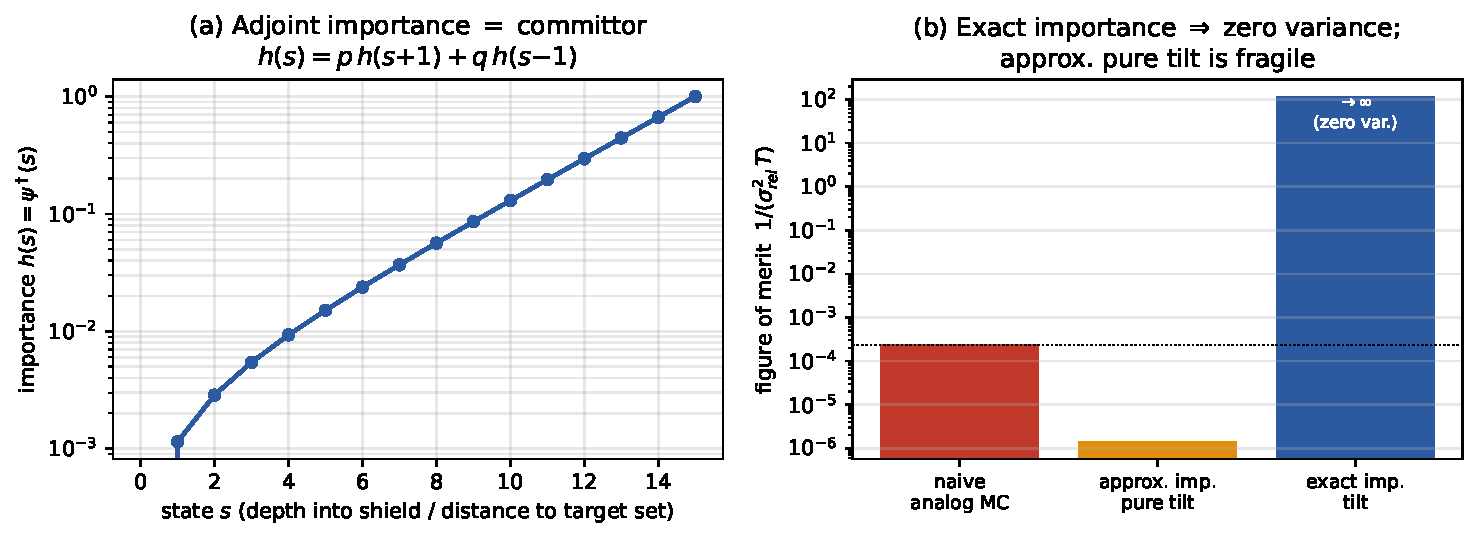
\includegraphics[width=0.92\textwidth]{figs/committor_demo.pdf}
\caption{Exact demonstration of \S\ref{sec:identity} (computed). A nearest-neighbour walk on
$\{0,\dots,15\}$ drifts toward $0$; reaching $15$ first is the rare deep-penetration event,
$\pi=1.14\times10^{-3}$. (a) The importance $h(s)=\psi\dg(s)$ rises steeply toward the target
and obeys the adjoint equation \eqref{eq:committor}. (b) Figure of merit. Naive analog Monte
Carlo (red) is the baseline; tilting \eqref{eq:tilt} with the \emph{exact} importance (blue)
gives measured relative variance $\sim\!10^{-30}$ --- zero variance to machine precision;
tilting with an \emph{approximate} importance under \emph{pure biasing} (amber) is
\emph{worse than doing nothing}. That fragility is exactly why deep-penetration transport
uses weight windows (split/roulette) to bound the weights --- the robustness layer whose
gain on spin systems Phase 2 will quantify.}
\label{fig:demo}
\end{figure}

\section{The dictionary}
Table~\ref{tab:dict} is the correspondence, with each row marked \textbf{[E]} exact
(a theorem-level identity) or \textbf{[H]} heuristic (a useful but non-rigorous analogy).

\begin{table}[h]
\centering\small
\caption{Radiation-transport variance reduction $\leftrightarrow$ neural rare-event sampling.}
\label{tab:dict}
\renewcommand{\arraystretch}{1.25}
\begin{tabular}{@{}p{4.9cm}p{6.4cm}c@{}}
\toprule
\textbf{Transport (deep penetration)} & \textbf{Neural sampler (rare events in stat.\ mech.)} & \\
\midrule
Adjoint flux / importance $\psi\dg(P)$ & Committor $h(s)$; learned importance $I_\theta(s)$ & [E]\\
Adjoint equation $\mathcal H\dg\psi\dg=\sigma_d$ & Backward/committor eqn.\ $(\mathbb I-K)h=0$, target $=$ adjoint source & [E]\\
Fundamental identity $R=\ip{\psi\dg}{q}$ & $\pi=\E_{p}[\mathbf 1_B]=h(s_0)$ & [E]\\
Importance-weighted zero-variance scheme & Doob / committor-tilted zero-variance sampler \eqref{eq:tilt} & [E]\\
Weight-window target $w\propto1/\psi\dg$ & Bounded importance weights $w\propto1/h$ & [E]\\
Splitting / Russian roulette & Branching / resampling of configurations (robustness layer) & [E]\\
CADIS: cheap adjoint drives forward MC & Cheap/learned $I_\theta$ drives the neural proposal & [H]\\
Source--weight-window consistency condition & Proposal must match the weight map or weights blow up & [E]\\
FW-CADIS: uniform relative error, all tallies & Uniform error across a family of tails / whole $I(a)$ & [H]\\
Figure of merit $1/(\sigma_{\mathrm{rel}}^2T)$ & Training objective for the sampler & [E]\\
Static equilibrium flux & Static Gibbs sampling & [H]\\
\bottomrule
\end{tabular}
\end{table}

\section{Consequences the ML literature is not using}

\paragraph{The FOM is the right objective, not reverse-KL.} Reverse-KL trains $q_\theta$ to
match the \emph{whole} Boltzmann distribution $p$. But the zero-variance sampler for a rare
tail is not $p$; it is the tilted measure $p(s)\,h(s)/\pi$, concentrated on the
configurations that realise the event. Training a VAN by minimising the \emph{relative
variance} of the tail estimator --- equivalently maximising the FOM --- targets that tilted
measure directly. This is a concrete, implementable change of loss with a transport
pedigree, and it sidesteps the known failure of global density matching for rare events.

\paragraph{The consistency condition is a design principle, not an afterthought.} The demo's
amber bar is the ML community's recurring ``importance sampling made it worse'' failure. In
transport it has a name and a fix: keep the proposal (source biasing) consistent with the
weight map, and bound weights with windows. Porting this discipline to neural proposals is
low-risk and directly useful.

\paragraph{Global variance reduction is untouched.} Every neural rare-event method we found
optimises \emph{one} event or rate. FW-CADIS's signature --- one importance map giving
uniform relative error across a whole family of targets (e.g.\ the entire large-deviation
curve $I(m)$ of the magnetisation) --- has no neural counterpart. This is the single most
defensible technical gap.

\section{Positioning against the two closest works}
\label{sec:pos}
\textbf{Kim \& Cai, arXiv:2602.12294 (Jan 2026)} --- the dangerous near-competitor --- learns
an importance function $I(s)$, modifies transitions as $K'(i\to j)=K(i\to j)I(j)/I(i)$, uses
a bias potential $E_b=-2k_BT\ln I$, and a branching random walk. In the language above:
their $I$ is our $h=\psi\dg$; their $K'$ is the tilt \eqref{eq:tilt}; their $E_b$ is the
weight-window target in energy units; their branching is splitting. They reconstructed the
zero-variance/weight-window recipe for discrete rare transitions --- \emph{without the
transport framing}. What they do \emph{not} do, and what remains open: the transport FOM as
objective; the \emph{global} FW-CADIS uniform-error goal; application to the spin-system
Boltzmann tails; a VAN (autoregressive, exactly-normalised) ansatz; and the consistency
condition as a stated design principle.

\smallskip
\noindent\textbf{Doob-transform VAN, Phys.\ Rev.\ E \textbf{111}, 034120 (2025)} approximates
the leading eigenvector of the \emph{tilted generator} with a VAN for \emph{dynamical} large
deviations. That eigenvector is the dynamical analogue of $\psi\dg$. What remains open:
static rare-event tails; the CADIS/weight-window robustness layer; the FOM objective; and
global (multi-target) variance reduction.

\section{What survives, and the bridge to Phase 2}
Three claims survive the prior-art check and are worth building:
\begin{enumerate}
\item \textbf{Unification (framing).} Identify $\psi\dg=h=I_\theta$ and place the recent
neural rare-event methods inside 70-year-old transport variance-reduction theory, importing
weight-window generators, the consistency condition, and the FOM wholesale.
\item \textbf{Global FW-CADIS for spin systems (headline).} One learned importance map that
equalises relative error across a family of magnetisation/energy tail thresholds --- the
whole rate function $I(m)$ --- rather than a single event.
\item \textbf{FOM-trained sampler.} Train the VAN/importance map by maximising
$1/(\sigma_{\mathrm{rel}}^2 T)$ under the consistency condition, and show robustness where
pure tilting (and reverse-KL) fail.
\end{enumerate}

\noindent\textbf{Phase 2 experiments that convert framing into a result.} On the 2D Ising
model (exact Onsager / Ferdinand--Fisher references available): (i) learn an approximate
committor/importance for a rare magnetisation tail; (ii) build FW-CADIS-style global weight
windows across a family of thresholds; (iii) measure the FOM against two baselines --- a
reverse-KL VAN with importance reweighting, and a single-target Kim--Cai-style biasing ---
with the \emph{global uniform-error} advantage as the headline metric; (iv) repeat on the
Edwards--Anderson spin glass to show the weight-window robustness layer survives a rugged
landscape (where the PNAS 2024 result shows plain neural samplers struggle). A positive FOM
gain of even $2$--$5\times$ at fixed cost, \emph{plus} the global-error property, clears
\textit{Mach.\ Learn.: Sci.\ Technol.} or \textit{Phys.\ Rev.\ E}; a demonstrated 3D or
spin-glass generalisation reaches for a stronger venue.

\paragraph{Immediate next action.} Nothing here needs new code. The single most valuable
Phase-2 seed is the exactly-solvable committor demo of Fig.~\ref{fig:demo}, extended one
step: add the weight-window (split/roulette) layer and show it recovers robust variance
reduction from an \emph{approximate} importance --- turning the amber bar green. That is a
half-day of work on the 1D model and becomes the controlled unit test for the 2D-Ising
implementation.

\section*{Key references}
\addcontentsline{toc}{section}{Key references}
\small
\begin{enumerate}[itemsep=1pt]
\item D.\ Wu, L.\ Wang \& P.\ Zhang, \emph{Solving statistical mechanics using variational autoregressive networks}, Phys.\ Rev.\ Lett.\ \textbf{122}, 080602 (2019); arXiv:1809.10606.
\item M.\ Kim \& W.\ Cai, \emph{Accelerated MCMC via neural network-driven importance sampling}, arXiv:2602.12294 (2026). [closest prior art]
\item \emph{Nonequilibrium statistical mechanics revealed by Doob transform and variational autoregressive networks}, Phys.\ Rev.\ E \textbf{111}, 034120 (2025).
\item J.\ C.\ Wagner \& A.\ Haghighat, \emph{Automated variance reduction of Monte Carlo shielding calculations using the discrete ordinates adjoint function} (CADIS), Nucl.\ Sci.\ Eng.\ \textbf{128}, 186--208 (1998).
\item J.\ C.\ Wagner, D.\ E.\ Peplow \& S.\ W.\ Mosher, \emph{FW-CADIS method for global and regional variance reduction\dots}, Nucl.\ Sci.\ Eng.\ \textbf{176}, 37--57 (2014).
\item M.\ A.\ Cooper \& E.\ W.\ Larsen, \emph{Automated weight windows for global Monte Carlo particle transport}, Nucl.\ Sci.\ Eng.\ \textbf{137}, 1--13 (2001).
\item K.\ A.\ Nicoli et al., \emph{Asymptotically unbiased estimation of physical observables with neural samplers}, Phys.\ Rev.\ E \textbf{101}, 023304 (2020).
\item D.\ Wu, R.\ Rossi \& G.\ Carleo, \emph{Unbiased Monte Carlo cluster updates with autoregressive neural networks}, Phys.\ Rev.\ Research \textbf{3}, L042024 (2021).
\item W.\ E \& E.\ Vanden-Eijnden, \emph{Towards a theory of transition paths} / transition-path theory (committor formalism), J.\ Stat.\ Phys.\ \textbf{123}, 503 (2006).
\item J.\ Spanier \& E.\ M.\ Gelbard, \emph{Monte Carlo Principles and Neutron Transport Problems} (1969) --- classical zero-variance / importance theory.
\end{enumerate}

\end{document}
